\documentclass{beamer}
\usepackage{etex}
\usepackage[utf8]{inputenc}
\usepackage[T1]{fontenc}
\usepackage{amssymb}
\usepackage{color}
\usepackage{verbatim}
\usepackage{beamerthemesplit}
\usepackage{graphicx}
\usepackage{xspace}
\usepackage{algorithm}
\usepackage{listings}
\usepackage{figlatex}
\usepackage{algorithmic}
\usepackage{multirow}
\usepackage{alltt}

\beamertemplatetransparentcovereddynamic

%\setbeamertemplate{background canvas}[vertical shading][bottom=red!10,top=blue!10]
%\usetheme{Warsaw}

\usepackage{../style/beamercolorthemeprogressbar}
\usepackage{../style/beamerfontthemeprogressbar}
\usepackage{../style/beamerouterthemeprogressbar}
\usepackage{../style/beamerinnerthemeprogressbar}

\setbeamertemplate{navigation symbols}{}
\beamertemplatetransparentcovereddynamic

\definecolor{javared}{rgb}{0.6,0,0} % for strings
\definecolor{javagreen}{rgb}{0.30,0.55,0.40} % comments
\definecolor{javapurple}{rgb}{0.5,0,0.35} % keywords
\definecolor{javadocblue}{rgb}{0.25,0.35,0.75} % java


\lstdefinestyle{BOAST}{
  language=Ruby,
  basicstyle=\tiny\ttfamily,
  keywordstyle=\color{javapurple}\bfseries,
  stringstyle=\color{javared},
  commentstyle=\color{javagreen},
  backgroundcolor=\color{white},
  numbers=left,
  morekeywords={BOAST, pr, decl, opn, close, For, Procedure, Real, Int, If, out, inout, Dim}
}
\lstdefinestyle{BFortran}{
  language=Fortran,
  basicstyle=\tiny\ttfamily,
  keywordstyle=\color{javapurple}\bfseries,
  stringstyle=\color{javared},
  commentstyle=\color{javagreen},
  numbers=left,
  tabsize=4,
  showspaces=false,
  showstringspaces=false
}
\lstdefinestyle{BC}{
  language=C,
  basicstyle=\tiny\ttfamily,
  keywordstyle=\color{javapurple}\bfseries,
  stringstyle=\color{javared},
  commentstyle=\color{javagreen},
  numbers=left,
  tabsize=4,
  showspaces=false,
  showstringspaces=false,
  morekeywords={kernel, global, uchar, short16, uchar16, int16, int32\_t, int64\_t},
}

\graphicspath{{../figures/}}

\title{BOAST}
\subtitle{Performance Portability Using Meta-Programming and Auto-Tuning}
\author[B. V.]{\textbf{Brice~Videau}~\inst{2}, Kevin~Pouget~\inst{1}, Luigi~Genovese~\inst{2},
                    Thierry~Deutsch~\inst{2}, Julien Bigot~\inst{5}, Guillaume Latu~\inst{4}, Virginie Grandgirard~\inst{4}, Dimitri~Komatitsch~\inst{3}, Fr\'ed\'eric~Desprez~\inst{1}, Jean-François~Méhaut~\inst{1}}
\institute[CNRS]{\inst{1} INRIA/LIG - CORSE,
                 \inst{2} CEA - L\_Sim,
                 \inst{3} CNRS,
                 \inst{4} CEA - IRFM,
                 \inst{5} CEA - Maison de la Simulation}

\date{\textbf{CEA - RIKEN Summer School, Kobe}\\July 6, 2018}

%\logo{
%   
\includegraphics[scale=.09]{logo_eocoe}
%   }

\bibliographystyle{plain}
\begin{document}

\frame{\titlepage}

\section{Introduction}

\subsection{Context}

\begin{frame}
  \frametitle{Scientific Application Portability}

  \begin{block}{\footnotesize Limited Portability}
    \begin{itemize}
      \item \scriptsize Huge codes (more than 100 000 lines), Written in FORTRAN or C++
      \item \scriptsize Collaborative efforts
      \item \scriptsize Use many different programming paradigms (OpenMP, OpenCL, CUDA, ...)
    \end{itemize}
  \end{block}

  \begin{columns}

  \column{0.45\linewidth}
  \begin{block}{\footnotesize But Based on \emph{Computing Kernels}}
    \begin{itemize}
      \item \scriptsize Well defined parts of a program
      \item \scriptsize Compute intensive
      \item \scriptsize Prime target for optimization
    \end{itemize}
  \end{block}

  \column{0.58\linewidth}
  \begin{block}{\footnotesize Kernels Should Be Written}
    \begin{itemize}
      \item \scriptsize In a \emph{portable} manner
      \item \scriptsize In a way that raises developer \emph{productivity}
      \item \scriptsize To present good \emph{performance}
    \end{itemize}
  \end{block}

  \end{columns}

\end{frame}

\begin{frame}
  \frametitle{HPC Architecture Evolution}

  \begin{columns}

  \column{0.6\linewidth}
  \begin{block}{\footnotesize Very Rapid and Diverse, Top500:}
    \begin{itemize}
      \item \scriptsize IBM Power 9 + nVidia GPU (Summit)
      \item \scriptsize Sunway processor (TaihuLight)
      \item \scriptsize Intel processor + Xeon Phi (Tianhe-2)
      \item \scriptsize AMD processor + nVidia GPU (Titan)
      \item \scriptsize IBM BlueGene/Q (Sequoia)
      \item \scriptsize Fujitsu SPARC64 (K Computer)
      \item \scriptsize Intel processor + nVidia GPU (Tianhe-1)
      \item \scriptsize AMD processor (Jaguar)
    \end{itemize}
  \end{block}

  \column{0.4\linewidth}
  \begin{block}{\footnotesize Tomorrow?}
    \begin{itemize}
      \item \scriptsize ARM + DSP?
      \item \scriptsize Intel Atom + FPGA?
      \item \scriptsize Quantum computing?
    \end{itemize}
  \end{block}

  \end{columns}

  \vspace{1cm}
  How to write kernels that could adapt to those architectures?\\
  (well maybe not quantum computing...)

\end{frame}

\subsection{Related Work}

\begin{frame}
  \frametitle{Related Work}

  \begin{itemize}
    \item \textbf{Ad hoc autotuners (usually for libraries):}
    \begin{itemize}
      \item \textbf{Atlas}~\cite{whaley04} (C macro processing)
      \item \textbf{SPIRAL}~\cite{puschel2004spiral} (DSL)
      \item ...
    \end{itemize}
    \item \textbf{Generic frameworks using annotation systems:}
    \begin{itemize}
      \item \textbf{POET}~\cite{yi2007poet} (external annotation file)
      \item \textbf{Orio}~\cite{Hart2009:Orio} (source annotation)
      \item \textbf{BEAST}~\cite{CPE:CPE3516} (Python preprocessor based, embedded DSL for optimization space definition/pruning)
    \end{itemize}
    \item \textbf{Generic frameworks using embedded DSL:}
    \begin{itemize}
      \item \textbf{Halide}~\cite{ragan2013halide} (C++, not very generic, 2D stencil targeted)
      \item \textbf{Heterogeneous Programming Library}~\cite{F.Fabeiro:2016:WPM:2894387.2894576} (C++)
    \end{itemize}
  \end{itemize}

\end{frame}

\section{A Parametrized Generator}
\begin{frame}
\frametitle{BOAST: a Parametrized Generator}
\end{frame}

\subsection{Motivation and Principles}

\begin{frame}

  \frametitle{Classical Tuning of Computing Kernels}

  \begin{center}%
    \includegraphics<1>[scale=1]{Workflow1-1}%
    \includegraphics<2>[scale=1]{Workflow1-2}%
    \includegraphics<3>[scale=1]{Workflow1-3}%
    \includegraphics<4>[scale=1]{Workflow1-4}%
  \end{center}%
  \begin{itemize}%
\only<1>{    \item Kernel optimization workflow}%
\only<1>{    \item Usually performed by a knowledgeable developer}%
\only<2>{    \item Compilers perform optimizations}%
\only<2>{    \item Architecture specific or generic optimizations}%
\only<3>{    \item Performance data hint at source transformations}%
\only<3>{    \item Architecture specific or generic hints}%
\only<4>{    \item Multiplication of kernel versions and/or loss of versions}%
\only<4>{    \item Difficulty to benchmark versions against each-other}%
  \end{itemize}%

\end{frame}

\begin{frame}
  \frametitle{BOAST Workflow \vphantom{Cp}}
  \begin{center}
    \includegraphics<1>[scale=1]{Workflow2-1}
    \includegraphics<2>[scale=1]{Workflow2-2}
    \includegraphics<3>[scale=1]{Workflow2-3}
  \end{center}
  \begin{itemize}%
\only<1>{    \item Meta-programming of optimizations in BOAST }
\only<1>{    \item High level object oriented language }
\only<2>{    \item Generate combination of optimizations }
\only<2>{    \item C, OpenCL, FORTRAN and CUDA are supported }
\only<3>{    \item Compilation and analysis are automated }
\only<3>{    \item Selection of best version can also be automated \vphantom{Cp}}
  \end{itemize}%
\end{frame}

\begin{frame}
\frametitle{BOAST Architecture}
 \begin{center}
   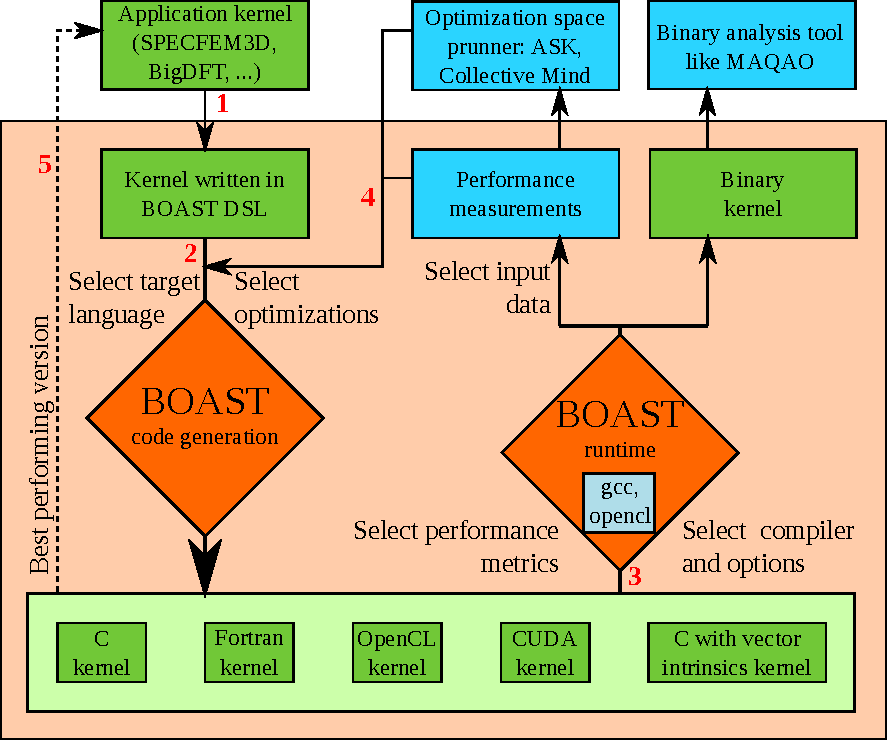
\includegraphics[scale=0.5]{BOAST_Workflow}
 \end{center}
\end{frame}

\subsection{EDSL}

\begin{frame}[fragile]
\frametitle{Motivating Example: BigDFT's MagicFilter}
The simplest convolution found in BigDFT, corresponds to the potential operator.
\begin{columns}
\column{4cm}
\begin{block}{Characteristics}
\begin{itemize}
\item Separable,
\item Filter length 16,
\item Transposition,
\item Periodic,
\item Only 32 operations per element.
\end{itemize}
\end{block}
\column{6.2cm}
\begin{block}{Pseudo code}
\lstset{style=BC}
\begin{lstlisting}
double filt[16] = {F0, F1, ... , F15};
void magicfilter(int n, int ndat, 
                 double *in, double *out){
  double temp;
  for(j = 0; j < ndat; j++) {
    for(i = 0; i < n; i++) {
       temp = 0;
       for(k = 0; k < 16; k++) {
         temp += in[ ((i-7+k)\%n) + j*n] 
                  * filt[k];
       }
       out[j + i*ndat] = temp;
} } }
\end{lstlisting}
\end{block}
\end{columns}
\end{frame}

\begin{frame}
\frametitle{Use Case Driven}
Parameters arising in a convolution:
\begin{itemize}
\item Filter: length, values, center.
\item Direction: forward or inverse convolution.
\item Boundary conditions: free or periodic.
\item Unroll factor: arbitrary.
\end{itemize}
How are those parameters constraining our tool?
\end{frame}

\begin{frame}
\frametitle{Features required}
Unroll factor:
\begin{itemize}
\item Create and manipulate an unknown number of variables,
\item Create loops with variable steps.
\end{itemize}
Boundary conditions:
\begin{itemize}
\item Manage arrays with parametrized size.
\end{itemize}
Filter and convolution direction:
\begin{itemize}
\item Transform arrays.
\end{itemize}
And of course be able to describe convolutions and output them in different languages.
\end{frame}

\begin{frame}
\frametitle{Proposed Generator}
Idea: use a high level language with support for operator overloading to describe the structure of the code, rather than trying to transform a decorated tree.\\
Define several abstractions:
\begin{itemize}
\item Variables: type (array, float, integer), size...
\item Operators: affect, multiply...
\item Procedure and functions: parameters, variables...
\item Constructs: for, while...
\end{itemize}
\end{frame}

\begin{frame}[fragile]
\frametitle{Sample Code: Variables and Parameters}
\lstset{style=BOAST}
\begin{lstlisting}
  #simple Variable
  i = Int "i"
  #simple constant
  fil_length = 16
  fil_center = 8  
  lowfil = Int( "lowfil", :const => -center )
  upfil = Int( "upfil", :const => length - center - 1 )
  #simple constant array
  arr = [F1, F2, ... , F16]
  fil = Real("fil", :const => arr, :dim => [ Dim(lowfil,upfil) ])
  #simple parameters
  n = Int( "n", :dir => :in)
  ndat = Int("ndat", :dir => :in)
  #array parameters
  x = Real("x", :dir => :in, :dim => [ Dim(0, n-1), Dim(ndat) ] )
  #multidimensional array, an output parameter
  y = Real("y", :dir => :out, :dim => [ Dim(ndat), Dim(0, n-1) ] )
\end{lstlisting}
Variables and Parameters are objects with a name, a type, and a set of named properties.
\end{frame}

\begin{frame}[fragile]
\frametitle{Sample Code: Keywords}
We need keywords to translate our expressions into code:
\begin{itemize}
\item \emph{pr}: print an expression or a construct
\item \emph{decl}: declare a variable or procedure
\item \emph{opn}: open a procedure or construct
\item \emph{close}: close a procedure or construct
\end{itemize}
\begin{columns}
\column{0.3\textwidth}
BOAST
\lstset{style=BOAST}
\begin{lstlisting}
i = Int "i"
k = Int "k", :size => 8
decl i, k
pr i === 5
j = (i + 5) * 2
pr k === j
\end{lstlisting}
\column{0.3\textwidth}
FORTRAN
\lstset{style=BFortran}
\begin{lstlisting}
integer(kind=4) :: i
integer(kind=8) :: k
i = 5
k = (i + 5) * (2)
\end{lstlisting}
\column{0.3\textwidth}
C
\lstset{style=BC}
\begin{lstlisting}
int32_t i;
int64_t k;
i = 5;
k = (i + 5) * (2);
\end{lstlisting}
\end{columns}
\end{frame}

\begin{frame}[fragile]
\frametitle{Sample Code: Procedure Declaration}
The following declaration:
\lstset{style=BOAST}
\begin{lstlisting}
p = Procedure("magicfilter", [n,ndat,x,y], :constants => [lowfil,upfil])
opn p
close p
\end{lstlisting}
Outputs Fortran:
\lstset{style=BFortran}
\begin{lstlisting}
subroutine magicfilter(n, ndat, x, y)
  integer(kind=4), parameter :: lowfil = -8
  integer(kind=4), parameter :: upfil = 7
  integer(kind=4), intent(in) :: n
  integer(kind=4), intent(in) :: ndat
  real(kind=8), intent(in), dimension(0:n-1, ndat) :: x
  real(kind=8), intent(out), dimension(ndat, 0:n-1) :: y
end procedure magicfilter
\end{lstlisting}
Or C:
\lstset{style=BC}
\begin{lstlisting}
void magicfilter(const int32_t n, const int32_t ndat, const double * x, double * y){
  const int32_t lowfil = -8;
  const int32_t upfil = 7;
}
\end{lstlisting}
\end{frame}

\begin{frame}[fragile]
\frametitle{Sample Code: Constructs and Arrays}
The following declaration:
\lstset{style=BOAST}
\begin{lstlisting}
  unroll = 5
  tt = unroll.times { |m| Real "tt#{m}" }
  pr For(j,1,ndat-(unroll-1), step: unroll) {
  #.....
    unroll.times { |m|
      pr tt[m] === tt[m] + x[k,j+m]*fil[l]
    }
  #.....
  }
\end{lstlisting}
\begin{columns}
\column{.35\textwidth}
Outputs Fortran:
\lstset{style=BFortran}
\begin{lstlisting}
  do j=1, ndat-4, 5
    !......
    tt0=tt0+x(k,j+0)*fil(l)
    tt1=tt1+x(k,j+1)*fil(l)
    tt2=tt2+x(k,j+2)*fil(l)
    tt3=tt3+x(k,j+3)*fil(l)
    tt4=tt4+x(k,j+4)*fil(l)
    !......
  enddo
\end{lstlisting}
\column{.65\textwidth}
Or C:
\lstset{style=BC}
\begin{lstlisting}
  for(j=1; j<=ndat-4; j+=5){
  /*...........*/
    tt0=tt0+x[k-0+(j+0-1)*(n-1-0+1)]*fil[l-lowfil];
    tt1=tt1+x[k-0+(j+1-1)*(n-1-0+1)]*fil[l-lowfil];
    tt2=tt2+x[k-0+(j+2-1)*(n-1-0+1)]*fil[l-lowfil];
    tt3=tt3+x[k-0+(j+3-1)*(n-1-0+1)]*fil[l-lowfil];
    tt4=tt4+x[k-0+(j+4-1)*(n-1-0+1)]*fil[l-lowfil];
  /*...........*/
  }
\end{lstlisting}
\end{columns}
\end{frame}

\begin{frame}[fragile]
\frametitle{BOAST is a State Machine}
  Changing BOAST state changes BOAST's output:
  \vskip 1em
\begin{columns}
\column{0.5\textwidth}
BOAST:
\lstset{style=BOAST}
\begin{lstlisting}
block = lambda {
  a = Real "a"
  b = Real "b", dim: Dim(10)
  decl a,b
  pr a === 5.0
  pr b[3] === a
}
push_env( :lang => FORTRAN,
          :array_start => 0 )
block.call
pop_env( :lang, :array_start)

push_env( :lang => C,
          :default_real_size => 4) {
  block.call
}
\end{lstlisting}
\column{0.5\textwidth}
outputs:
\lstset{style=BFortran}
\begin{lstlisting}
real(kind=8) :: a
real(kind=8), dimension(0:9) :: b
a = 5.0_wp
b(3) = a
\end{lstlisting}
\lstset{style=BC}
\begin{lstlisting}
float a;
float * b;
a = 5.0f;
b[3 - (1)] = a;
\end{lstlisting}
\end{columns}
\end{frame}

\begin{frame}[fragile]
\frametitle{OpenMP}
  All OpenMP constructs are supported. Simple BOAST sample:
\lstset{style=BOAST}
\begin{lstlisting}
n = Int("n", :dir => :in)
a = Real("a", :dir => :in, :dim => [Dim(0, n - 1)])
b = Real("b", :dir => :inout , :dim => [Dim(0, n - 1)])
pr p = Procedure("vector_add", [n, a , b]) {
  decl( i = Int("i") )
  pr OpenMP::Parallel(:private => [i], :shared => [a,b]) {
    pr For(i, 0, n - 1, :openmp => true) {
      pr b[i] === b[i] + a[i]
    }
  }
}
\end{lstlisting}
\begin{columns}
\column{0.65\textwidth}
FORTRAN
\lstset{style=BFortran}
\begin{lstlisting}
SUBROUTINE vector_add(n, a, b)
  integer, parameter :: wp=kind(1.0d0)
  integer(kind=4), intent(in) :: n
  real(kind=8), intent(in), dimension(0:n-1) :: a
  real(kind=8), intent(inout), dimension(0:n-1) :: b
  integer(kind=4) :: i
!$omp parallel  private(i) shared(a, b)
!$omp do 
  do i = 0, n - (1), 1
    b(i) = b(i) + a(i)
  end do
!$omp end do 
!$omp end parallel 
END SUBROUTINE vector_add
\end{lstlisting}
\column{0.35\textwidth}
C
\lstset{style=BC}
\begin{lstlisting}
void vector_add(const int32_t n,
                const double * a,
                double * b){
  int32_t i;
#pragma omp parallel \
  private(i) shared(a, b)
{
#pragma omp for 
  for (i = 0; i <= n-(1); i += 1)
  {
    b[i] = b[i] + a[i];
  }
}
}
\end{lstlisting}
\end{columns}
\end{frame}

\begin{frame}[fragile]
\frametitle{Vector Programming}
Intrinsics supported in C, array notations used in FORTRAN.\\
BOAST:
\lstset{style=BOAST}
\begin{lstlisting}
vl = 4 ; nvec = Int "nvec"; i = Int "i"
a = Real( "a", :vector_length => vl, :dim => [Dim(nvec)] )
b = Real( "b", :vector_length => vl, :dim => [Dim(nvec)] )
c = Real( "c" )
tmp = Real "tmp", :vector_length => vl
pr tmp.set( 0.0 )
pr For( i, 0, nvec - 1 ) {
  pr tmp === tmp + a[i] * b[i]
}
pr c === vl.times.collect { |j| tmp[j] }.reduce(:+)
\end{lstlisting}
FORTRAN:
\lstset{style=BFortran}
\begin{lstlisting}
tmp = 0.0_wp
do i = 0, nvec - (1), 1
  tmp = tmp + (a(:, i)) * (b(:, i))
end do
c = tmp(1) + tmp(2) + tmp(3) + tmp(4)
\end{lstlisting}
C:
\lstset{style=BC}
\begin{lstlisting}
tmp = _mm256_setzero_pd( );
for (i = 0; i <= nvec - (1); i += 1) {
  tmp = _mm256_add_pd( tmp, _mm256_mul_pd( a[i - (1)], b[i - (1)] ) );
}
c = tmp[0] + tmp[1] + tmp[2] + tmp[3];
\end{lstlisting}
\end{frame}

\section{Case Studies}

\begin{frame}
\frametitle{Case Studies}
\end{frame}

\subsection{BigDFT}

\begin{frame}
  \frametitle{BigDFT}
  \begin{center}
    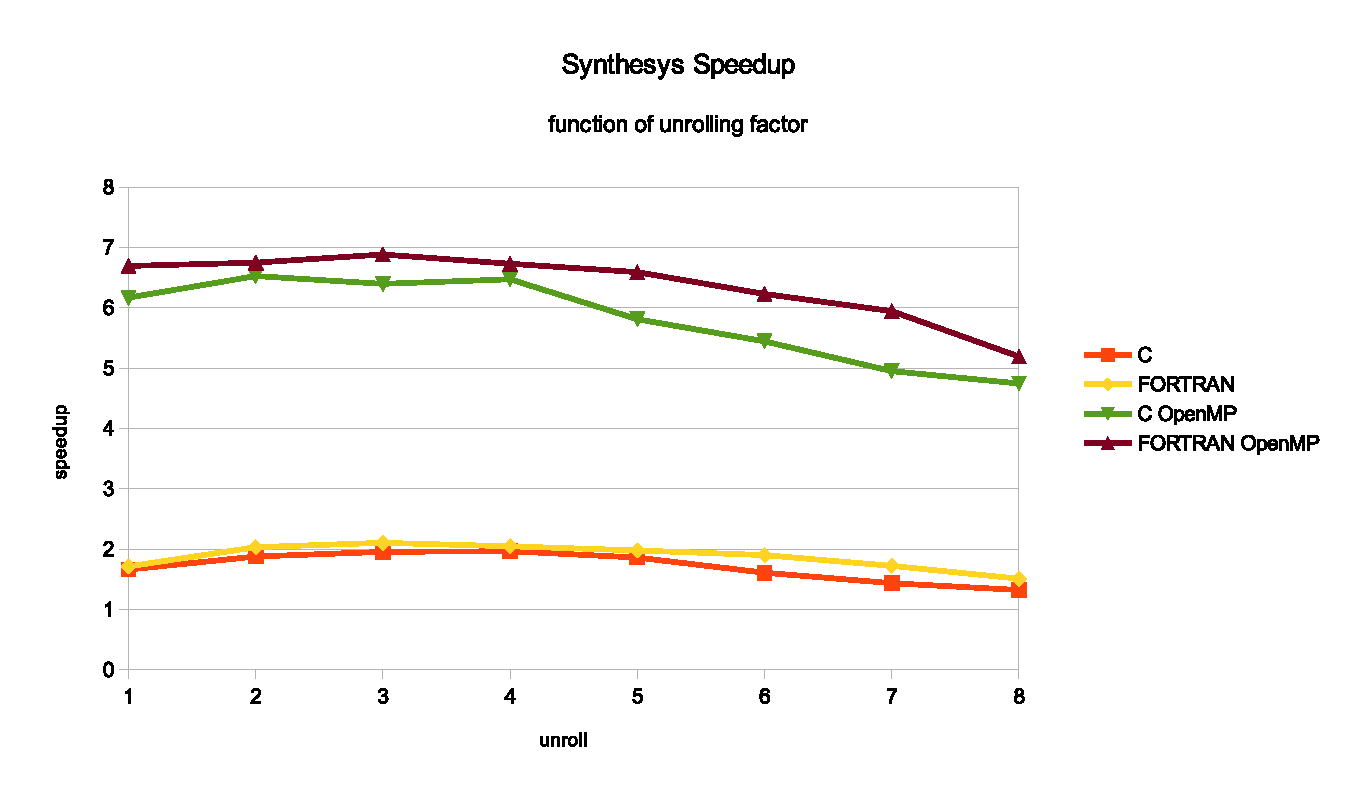
\includegraphics[scale=0.35]{Res_synthesis}
  \end{center}

 \begin{itemize}
  \item Novel approach for DFT computation based on Daubechies wavelets
  \item Fortran and C code, MPI, OpenMP, supports CUDA and OpenCL
   \item Reference is hand tuned code on target architecture (Nehalem)
    \item Toward a BLAS-like library for wavelets
  \end{itemize}
\end{frame}

\subsection{SPECFEM3D}

\begin{frame}
  \frametitle{SPECFEM3D}

  \begin{itemize}
   \item Seismic wave propagation simulator
    \item SPECFEM3D ported to OpenCL using BOAST
    \begin{itemize}
      \item Unified code base (CUDA/OpenCL)
      \item Refactoring: kernel code base reduced by 40\%
      \item Similar performance on NVIDIA Hardware
      \item Non regression test for GPU kernels
    \end{itemize}
    \item On the Mont-Blanc prototype:
    \begin{itemize}
      \item OpenCL+MPI runs
      \item Speedup of 3 for the GPU version
    \end{itemize}
  \end{itemize}
\end{frame}

\subsection{Laplacian}

\begin{frame}[fragile]
  \frametitle{Example: Laplace Kernel from ARM}
\lstset{style=BC}
\begin{lstlisting}
void laplace(const int width,
             const int height,
             const unsigned char src[height][width][3],
                   unsigned char dst[height][width][3]){
  for (int j = 1; j < height-1; j++) {
    for (int i = 1; i < width-1; i++) {
      for (int c = 0; c < 3; c++) {
        int tmp = -src[j-1][i-1][c] -   src[j-1][i][c] - src[j-1][i+1][c]\
                 - src[j  ][i-1][c] + 9*src[j  ][i][c] - src[j  ][i+1][c]\
                 - src[j+1][i-1][c] -   src[j+1][i][c] - src[j+1][i+1][c];
        dst[j][i][c] = (tmp < 0 ? 0 : (tmp > 255 ? 255 : tmp));
      }
    }
  }
}
\end{lstlisting}
\begin{itemize}
\item C reference implementation
\item Many opportunities for improvement
\item ARM GPU Mali 604 within the Montblanc project
\end{itemize}
\end{frame}


\begin{frame}[fragile]
  \frametitle{Example: Laplace in OpenCL}
\lstset{style=BC}
\begin{lstlisting}
kernel laplace(const int width,
               const int height,
               global const uchar *src,
               global       uchar *dst){
  int i = get_global_id(0);
  int j = get_global_id(1);
  for (int c = 0; c < 3; c++) {
    int tmp = -src[3*width*(j-1) + 3*(i-1) + c]\
             - src[3*width*(j-1) + 3*(i  ) + c]\
             - src[3*width*(j-1) + 3*(i+1) + c]\
             - src[3*width*(j  ) + 3*(i-1) + c]\
           + 9*src[3*width*(j  ) + 3*(i  ) + c]\
             - src[3*width*(j  ) + 3*(i+1) + c]\
             - src[3*width*(j+1) + 3*(i-1) + c]\
             - src[3*width*(j+1) + 3*(i  ) + c]\
             - src[3*width*(j+1) + 3*(i+1) + c];
    dst[3*width*j + 3*i + c] = clamp(tmp, 0, 255);
  }
}
\end{lstlisting}
\begin{itemize}
\item OpenCL reference implementation
\item Outer loops mapped to threads
\item 1 pixel per thread
\end{itemize}
\end{frame}

\begin{frame}[fragile]
  \frametitle{Example: Vectorizing}
\lstset{language=C,
basicstyle=\ttfamily,
keywordstyle=\color{javapurple}\bfseries,
morekeywords={kernel, global, uchar, uchar16, int16},
stringstyle=\color{javared},
commentstyle=\color{javagreen},
numbers=left,
tabsize=4,
showspaces=false,
showstringspaces=false}
\fontsize{3}{3}\selectfont
\begin{lstlisting}
kernel laplace(const int width,
               const int height,
               global const uchar *src,
               global       uchar *dst){
  int i = get_global_id(0);
  int j = get_global_id(1);
  uchar16 v11_ = vload16( 0, src + 3*width*(j-1) + 3*5*i - 3 );
  uchar16 v12_ = vload16( 0, src + 3*width*(j-1) + 3*5*i     );
  uchar16 v13_ = vload16( 0, src + 3*width*(j-1) + 3*5*i + 3 );
  uchar16 v21_ = vload16( 0, src + 3*width*(j  ) + 3*5*i - 3 );
  uchar16 v22_ = vload16( 0, src + 3*width*(j  ) + 3*5*i     );
  uchar16 v23_ = vload16( 0, src + 3*width*(j  ) + 3*5*i + 3 );
  uchar16 v31_ = vload16( 0, src + 3*width*(j+1) + 3*5*i - 3 );
  uchar16 v32_ = vload16( 0, src + 3*width*(j+1) + 3*5*i     );
  uchar16 v33_ = vload16( 0, src + 3*width*(j+1) + 3*5*i + 3 );
  int16 v11 = convert_int16(v11_);
  int16 v12 = convert_int16(v12_);
  int16 v13 = convert_int16(v13_);
  int16 v21 = convert_int16(v21_);
  int16 v22 = convert_int16(v22_);
  int16 v23 = convert_int16(v23_);
  int16 v31 = convert_int16(v31_);
  int16 v32 = convert_int16(v32_);
  int16 v33 = convert_int16(v33_);
  int16 res = v22 * (int)9 - v11 - v12 - v13 - v21 - v23 - v31 - v32 - v33;
        res = clamp(res, (int16)0, (int16)255);
  uchar16 res_ = convert_uchar16(res);
  vstore8(res_.s01234567, 0, dst + 3*width*j + 3*5*i);
  vstore8(res_.s89ab,     0, dst + 3*width*j + 3*5*i + 8);
  vstore8(res_.scd,       0, dst + 3*width*j + 3*5*i + 12);
  dst[3*width*j + 3*5*i + 14] = res_.se;
}
\end{lstlisting}
\begin{itemize}
\item Vectorized OpenCL implementation
\item 5 pixels instead of one (15 components)
\end{itemize}
\end{frame}

\begin{frame}[fragile]
  \frametitle{Example: Synthesizing Vectors}
\lstset{style=BC}
\begin{lstlisting}
uchar16 v11_ = vload16( 0, src + 3*width*(j-1) + 3*5*i - 3 );
uchar16 v12_ = vload16( 0, src + 3*width*(j-1) + 3*5*i     );
uchar16 v13_ = vload16( 0, src + 3*width*(j-1) + 3*5*i + 3 );
uchar16 v21_ = vload16( 0, src + 3*width*(j  ) + 3*5*i - 3 );
uchar16 v22_ = vload16( 0, src + 3*width*(j  ) + 3*5*i     );
uchar16 v23_ = vload16( 0, src + 3*width*(j  ) + 3*5*i + 3 );
uchar16 v31_ = vload16( 0, src + 3*width*(j+1) + 3*5*i - 3 );
uchar16 v32_ = vload16( 0, src + 3*width*(j+1) + 3*5*i     );
uchar16 v33_ = vload16( 0, src + 3*width*(j+1) + 3*5*i + 3 );
\end{lstlisting}
\centering Becomes
\begin{lstlisting}
uchar16 v11_ = vload16( 0, src + 3*width*(j-1) + 3*5*i - 3 );
uchar16 v13_ = vload16( 0, src + 3*width*(j-1) + 3*5*i + 3 );
uchar16 v12_ = uchar16( v11_.s3456789a, v13_.s56789abc );
uchar16 v21_ = vload16( 0, src + 3*width*(j  ) + 3*5*i - 3 );
uchar16 v23_ = vload16( 0, src + 3*width*(j  ) + 3*5*i + 3 );
uchar16 v22_ = uchar16( v21_.s3456789a, v23_.s56789abc );
uchar16 v31_ = vload16( 0, src + 3*width*(j+1) + 3*5*i - 3 );
uchar16 v33_ = vload16( 0, src + 3*width*(j+1) + 3*5*i + 3 );
uchar16 v32_ = uchar16( v31_.s3456789a, v33_.s56789abc );
\end{lstlisting}
\begin{itemize}
\item Reducing the number of loads since the vector are overlapping
\item Synthesizing loads should save bandwidth
\item Could be pushed further
\end{itemize}
\end{frame}

\begin{frame}[fragile]
  \frametitle{Example: Reducing Variable Size}
\lstset{style=BC}
\begin{lstlisting}
int16 v11 = convert_int16(v11_);
int16 v12 = convert_int16(v12_);
int16 v13 = convert_int16(v13_);
int16 v21 = convert_int16(v21_);
int16 v22 = convert_int16(v22_);
int16 v23 = convert_int16(v23_);
int16 v31 = convert_int16(v31_);
int16 v32 = convert_int16(v32_);
int16 v33 = convert_int16(v33_);
int16 res = v22 * (int)9 - v11 - v12 - v13 - v21 - v23 - v31 - v32 - v33;
      res = clamp(res, (int16)0, (int16)255);
\end{lstlisting}
\centering Becomes
\begin{lstlisting}
short16 v11 = convert_short16(v11_);
short16 v12 = convert_short16(v12_);
short16 v13 = convert_short16(v13_);
short16 v21 = convert_short16(v21_);
short16 v22 = convert_short16(v22_);
short16 v23 = convert_short16(v23_);
short16 v31 = convert_short16(v31_);
short16 v32 = convert_short16(v32_);
short16 v33 = convert_short16(v33_);
short16 res = v22 * (short)9 - v11 - v12 - v13 - v21 - v23 - v31 - v32 - v33;
        res = clamp(res, (short16)0, (short16)255);
\end{lstlisting}
\begin{itemize}
\item Using smaller intermediary types could save registers
\end{itemize}
\end{frame}

\begin{frame}
  \frametitle{Example: Optimization Summary}
  \begin{itemize}
    \item Very complex process (several other optimizations could be applied)
    \item Intimate knowledge of the architecture required
    \item Numerous versions to be benchmarked
    \item Difficult to test combination of optimizations:
    \begin{itemize}
      \item Vectorization,
      \item Intermediary data type,
      \item Number of pixels processed,
      \item Synthesizing loads.
    \end{itemize}
    \item Can we use BOAST to automate the process?
  \end{itemize}
\end{frame}

\begin{frame}
  \frametitle{Example: Laplace Kernel with BOAST}
  \begin{itemize}
    \item Based on components instead of pixel
    \item Use tiles rather than only sequence of elements
    \item Parameters used in the BOAST version:
    \begin{itemize}
      \item \emph{x\_component\_number}: a positive integer
      \item \emph{y\_component\_number}: a positive integer
      \item \emph{vector\_length}: 1, 2, 4, 8 or 16
      \item \emph{temporary\_size}: 2 or 4
      \item \emph{synthesizing\_loads}: true or false
    \end{itemize}
  \end{itemize}
\end{frame}

\begin{frame}
  \frametitle{Example: ARM results}
  \begin{center}
  \scriptsize
  \begin{tabular}{c|r|r|c|r|c}
    Image Size  & Naive (s) & Best (s) & Acceleration & BOAST (s) & Acceleration \\
    \hline&&&&\\
  768 x 432   & 0.0107    & 0.00669  & x1.6         & 0.000639  & x16.7 \\
  2560 x 1600 & 0.0850    & 0.0137   & x6.2         & 0.00687   & x12.4 \\
  2048 x 2048 & 0.0865    & 0.0149   & x5.8         & 0.00715   & x12.1 \\
  5760 x 3240 & 0.382     & 0.0449   & x8.5         & 0.0325    & x11.8 \\
  7680 x 4320 & 0.680     & 0.0747   & x9.1         & 0.0581    & x11.7
  \end{tabular}
  \end{center}

  \begin{itemize}
    \item Optimal parameter values:
    \begin{itemize}
      \item x\_component\_number: 16
      \item y\_component\_number: 1
      \item vector\_length: 16
      \item temporary\_size: 2
      \item synthesizing\_loads: false
    \end{itemize}
    \item Close to what ARM engineers found
  \end{itemize}
\end{frame}

\begin{frame}
  \frametitle{Example: Performance Portability}
  \begin{center}
  \scriptsize
  \begin{tabular}{c|r|r|c|r|c}
    Image Size & BOAST ARM (s) & BOAST Intel & Ratio & BOAST NVIDIA & Ratio \\
    \hline&&&&\\
  768 x 432   & 0.000639     & 0.000222    & x2.9  & 0.0000715    & x8.9  \\
  2560 x 1600 & 0.00687      & 0.00222     & x3.1  & 0.000782     & x8.8  \\
  2048 x 2048 & 0.00715      & 0.00226     & x3.2  & 0.000799     & x8.9  \\
  5760 x 3240 & 0.0325       & 0.0108      & x3.0  & 0.00351      & x9.3  \\
  7680 x 4320 & 0.0581       & 0.0192      & x3.0  & 0.00623      & x9.3
  \end{tabular}
  \end{center}

  \begin{columns}
  \column{0.5\textwidth}
  \begin{itemize}
    \item \footnotesize Optimal parameter values (Intel I7 2760, 2.4 GHz):
    \begin{itemize}
      \item \scriptsize x\_component\_number: 16
      \item \scriptsize y\_component\_number: 4..2
      \item \scriptsize vector\_length: 8
      \item \scriptsize temporary\_size: 2
      \item \scriptsize synthesizing\_loads: false
    \end{itemize}
  \end{itemize}
  \column{0.5\textwidth}
  \begin{itemize}
    \item \footnotesize Optimal parameter values nVidia (GTX 680):
    \begin{itemize}
      \item \scriptsize x\_component\_number: 4
      \item \scriptsize y\_component\_number: 4
      \item \scriptsize vector\_length: 4
      \item \scriptsize temporary\_size: 2
      \item \scriptsize synthesizing\_loads: false
    \end{itemize}
  \end{itemize}
  \end{columns}
  \vspace{1cm}
  \centering Performance \emph{portability} among several different architectures.
\end{frame}

\subsection{Gysela}

\begin{frame}
\frametitle{Gysela 2d Advection}
Gysela: Gyrokinetic Semi-Lagrangian\\
Tokamak plasma simulation for fusion (ITER)
\scalebox{0.9}{
\begin{minipage}{\textwidth}
\begin{itemize}
\item Preparation steps
\begin{itemize}
\item Extract 4 targeted routines from Gysela (subpart of 2d advection)
\item Change \textbf{API} of the 2d advection kernel\\
\hspace*{1cm} only arrays of integers and floats for inputs/outputs
\hspace*{1cm} (transmitting data structures is \textit{possible} but more \textit{complex})
\item Define  valid \textit{fake} inputs for  the kernel to  design a regression
  test
\item Integrate the reference/original version into BOAST
\end{itemize}
\item Install ruby \& BOAST on 4 parallel machines
\begin{itemize}
\item Easiest step
\item Get a working compilation/execution of the kernel: a bit more difficult
\end{itemize}
\item Write a meta-program that \textit{prints} a program
\begin{enumerate}
\item Need to learn a little bit of ruby \& BOAST
\item \textbf{Incremental approach: begin with internal routines then external}
\item Identify what are the \textit{parameters} of the auto-tuning
\item Integrate the best kernel version to the Gysela compilation process
\end{enumerate}
\end{itemize}
\end{minipage}
}
\end{frame}

\begin{frame}
\frametitle{Gysela 2d avection (2)}

\scalebox{1.}{
\begin{minipage}{\textwidth}
\begin{itemize}
\item Auto-tuning parameters that we chose
\begin{itemize}
\item directive based inlining / BOAST driven inlining
\item BOAST driven loop unrolling
\item C or Fortran code generated
\item scan versions of gfortran/gcc/icc/ifort (\texttt{module load})
\item loop blocking parameter (one of the most internal loop)
\item explicit vectorization: BOAST generates INTEL intrinsincs, e.g.
\scalebox{.6}{
\begin{minipage}{1.5\textwidth}
\begin{alltt}
ftmp1 = \_mm256\_setzero\_pd( );\\
ftmp2 = \_mm256\_setzero\_pd( );\\
ftmp1 = \_mm256\_fmadd\_pd(  base1[0], \_mm256\_load\_pd( \&ftransp[(0) * (4)]);\\
ftmp2 = \_mm256\_fmadd\_pd( base1[0 + 1], \_mm256\_load\_pd( \&ftransp[(0 + 1)  * (4)] ), ftmp2 );
\end{alltt}
\end{minipage}}
\end{itemize}
\medskip
\item Final result
\begin{itemize}
\item ruby code of 200 lines for the 2d advection kernel\\
\hspace*{1cm} compared to original fortran code of 300 lines
\medskip
\end{itemize}
\item Auto-tuning runs
\begin{itemize}
\item configure the list of modules/compilers for the \textit{parameter scan}
\item between 1 min and 20 min for the {parameter scan} on 1 machine
\end{itemize}
\end{itemize}
\end{minipage}}

\end{frame}

\begin{frame}
\frametitle{Auto-tuning on INTEL Westmere (2011)}
\begin{columns}
\column{.3\textwidth}
\scalebox{0.76}{
\begin{minipage}{6cm}
Auto-tuning for 2D advection\\
Computing center at Marseille\\
12-cores node -\\
\hspace*{.4cm} Intel X5675, 3.07GHz\\[1cm]
Nb of runs in this scan: 609\\
Runs sorted from quickest to slowest\\
Result of the scan \\
\hspace*{.4cm}\ (best parameters):\\[.2cm]
\end{minipage}
}
\scalebox{0.7}{
\begin{minipage}{6cm}
\begin{alltt}
:lang: FORTRAN\\
:unroll: true\\
:force.inline: true\\
:intrinsic: false\\
:blocking.size: 4\\
:module: intel/16.0.2\\
\end{alltt}

Speedup: \textcolor{red}{1.9}
\end{minipage}
}
\column{.70\textwidth}
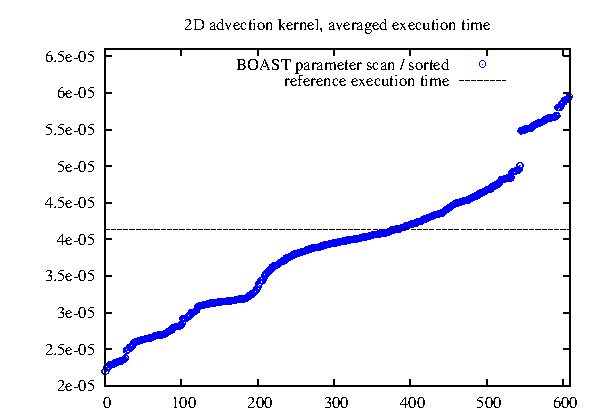
\includegraphics[width=1.0\textwidth]{rheticus.pdf}\\
\end{columns}
\end{frame}
  
\begin{frame}
\frametitle{Auto-tuning on INTEL Sandy-Bridge (2012)}
\begin{columns}
\column{.3\textwidth}
\scalebox{0.8}{
\begin{minipage}{6cm}
Auto-tuning for 2D advection\\
Computing center at Orsay\\
16-cores node - \\
\hspace*{0.4cm}Intel E5-2670 v1, 2.60GHz\\[1cm]
Result of the scan \\
\hspace*{.4cm}\ (best parameters):\\[.2cm]
\end{minipage}
}
\scalebox{0.7}{
\begin{minipage}{6cm}
\begin{alltt}
:lang: FORTRAN\\
:unroll: \textcolor{red}{false}\\
:force.inline: \textcolor{red}{false}\\
:intrinsic: false\\
:blocking.size: 2\\
:module: intel/15.0.0
\end{alltt}

Speedup: \textcolor{red}{1.7}
\end{minipage}
}
\column{.70\textwidth}
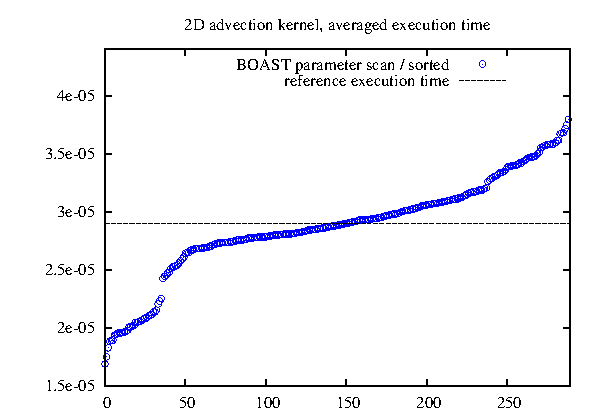
\includegraphics[width=1.0\textwidth]{poincare.pdf}\\
\end{columns}
\end{frame}
  
\begin{frame}
\frametitle{Auto-tuning on INTEL Haswell (2015)}
\begin{columns}
\column{.3\textwidth}
\scalebox{0.8}{
\begin{minipage}{6cm}
Auto-tuning for 2D advection\\
Computing center at Montpellier\\
24-cores node - \\
\hspace*{0.4cm}Intel E5-2690 v3, 2.60GHz\\[1cm]
Result of the scan \\
\hspace*{.4cm}\ (best parameters):\\[.2cm]
\end{minipage}
}
\scalebox{0.7}{
\begin{minipage}{6cm}
\begin{alltt}
:lang: FORTRAN\\
:unroll: true\\
:force.inline: true\\
:intrinsic: false\\
:blocking.size: 4\\
:module: \textcolor{red}{intel/14.0.4.211}\\
\end{alltt}

Speedup: \textcolor{red}{2.0}
\end{minipage}
}
\column{.70\textwidth}
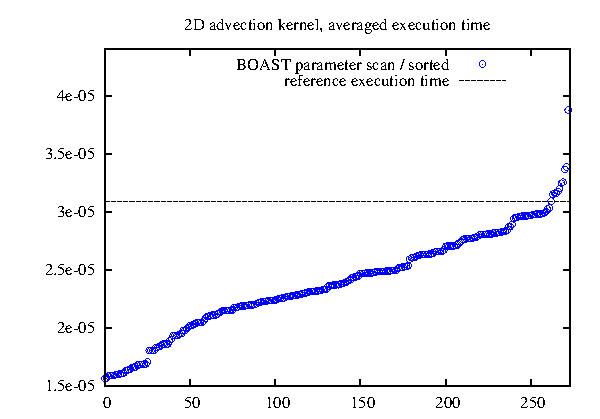
\includegraphics[width=1.0\textwidth]{occigen.pdf}\\
\end{columns}
\end{frame}

\begin{frame}
\frametitle{Auto-tuning on INTEL KNL (Phi 2016)}
\begin{columns}
\column{.3\textwidth}
\scalebox{0.8}{
\begin{minipage}{6cm}
Auto-tuning for 2D advection\\
Computing center at Montpellier\\
64-cores node - \\
\hspace*{0.4cm}Intel 7210  1.30GHz\\[1cm]
Result of the scan \\
\hspace*{.4cm}\ (best parameters):\\[.2cm]
\end{minipage}
}
\scalebox{0.7}{
\begin{minipage}{6cm}
\begin{alltt}
:lang: FORTRAN\\
:unroll: true\\
:force.inline: true\\
:intrinsic: false\\
:blocking.size: \textcolor{red}{32}\\
:module: \textcolor{red}{intel/17.0}\\
\end{alltt}

Speedup: \textcolor{red}{3.6}
\end{minipage}
}
\column{.70\textwidth}
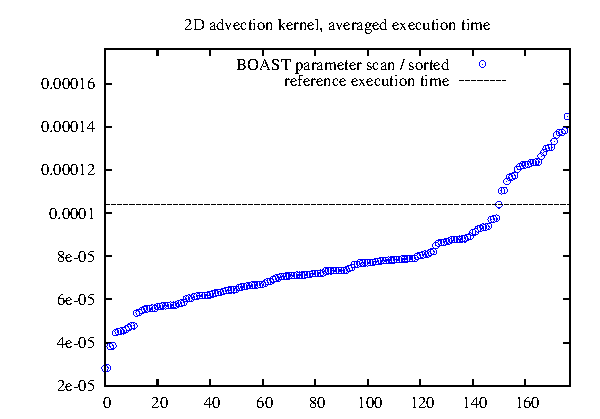
\includegraphics[width=1.0\textwidth]{knl.pdf}\\
\end{columns}
\end{frame}

\begin{comment}
\section{Real Applications}
\end{comment}

\section{Conclusions}

\begin{frame}
\frametitle{Conclusions and Perspectives}
\end{frame}

\begin{frame}
  \frametitle{Conclusions}
  \begin{itemize}
    \item BOAST v2.0 is released
    \item BOAST language features:
    \begin{itemize}
      \item Unified C and FORTRAN with OpenMP support,
      \item Unified OpenCL and CUDA support,
      \item Support for vector programming.
    \end{itemize}
    \item BOAST runtime features:
    \begin{itemize}
      \item Generation of parametric kernels,
      \item Parametric compilation,
      \item Non-regression testing of kernels,
      \item Benchmarking capabilities (PAPI support)
      \item Co-execution and numa-aware capabilities (using hwloc)
    \end{itemize}
  \end{itemize}
\end{frame}

\begin{frame}
  \frametitle{Perspectives}
  \begin{itemize}
    \item Ongoing work on other applications: Alya, dgtd\_nano3d
    \item Couple BOAST with other tools:
    \begin{itemize}
      \item Parametric space pruners (speed up optimization),
      \item Binary analysis (guide optimization, MAQAO),
      \item Source to source transformation (improve optimization),
      \item Binary transformation (improve optimization).
    \end{itemize}
    \item Improve BOAST:
    \begin{itemize}
      \item Improve the eDSL to make it more intuitive,
      \item Better vector support,
      \item Gather feedback.
    \end{itemize}
  \end{itemize}
\end{frame}


\begin{frame}
  \frametitle{And the Future?}
  New architectures:
  \begin{itemize}
    \item FPGAs:
    \begin{itemize}
      \item Supported via OpenCL,
      \item longer compile time,
      \item parallel compilation?
    \end{itemize}
    \item New vector architectures:
    \begin{itemize}
      \item Intel KNL and onward: masked vector instructions,
      \item ARM SVE: meta programming is in the instruction set.
    \end{itemize}
    \item New memory architectures:
    \begin{itemize}
      \item 3D stacked high performance memory (KNL, GPUs): new address space,
      \item Non Volatile RAM: new address space again (relevant for computing kernels?)?
    \end{itemize}
  \end{itemize}
\end{frame}
\section{Bibliography}

\begin{frame}[shrink=50]
  \frametitle{Bibliography}
  \bibliography{../biblio/BOAST}
\end{frame}

\end{document}
